% ===================================================================== CHƯƠNG 3
\chapter{Phát biểu bài toán và thiết kế giải pháp}\label{ch:thiet-ke}

Chương này trả lời hai câu hỏi: bài toán được phát biểu hình thức như thế nào, và hệ thống \tensp{} được thiết kế ra sao để giải bài toán đó. Mô tả bám theo mã nguồn tại ngày 09/11/2026. Chương chỉ nêu tham số cấu hình và lý do chọn; kết quả đo nằm ở Chương~\ref{ch:ket-qua}.

\section{Phát biểu bài toán}\label{sec:phat-bieu}

\subsection{Đầu vào}

Một lượt phân tích nhận một tập tài liệu. Mỗi tài liệu mang hai nhãn do người dùng chọn hoặc hệ thống gợi ý:
\begin{itemize}
\item \textbf{vai trò}: tài liệu đang được soát (nguồn tuyên bố), tài liệu đối chiếu, hoặc tài liệu tham chiếu chung;
\item \textbf{loại nguồn}: nội bộ doanh nghiệp, tài chính, môi trường, pháp lý, bên ngoài, chuẩn mực. Loại nguồn quyết định một đoạn văn có được coi là \emph{độc lập} với doanh nghiệp hay không.
\end{itemize}

Từ tài liệu nguồn, hệ thống rút ra tập tuyên bố. Mỗi tuyên bố là một câu, hoặc một phần câu sau khi tách câu nhiều mệnh đề có số, kèm năm thuộc tính: chỉ số, giá trị kèm đơn vị, kỳ báo cáo, năm gốc, phạm vi hoặc ranh giới. Thuộc tính nào câu không nêu thì để trống. Thiếu thuộc tính là một thông tin cho người soát, không phải lỗi.

\subsection{Đầu ra}

Với mỗi tuyên bố, hệ thống trả về một bản ghi gồm:
\begin{enumerate}
\item \textbf{một kết luận} trong năm loại (Bảng~\ref{tab:ket-luan});
\item \textbf{bằng chứng}: các đoạn văn kèm tên tài liệu, số trang, nguyên văn, quan hệ với tuyên bố và \emph{phương pháp} đã quyết định quan hệ đó (số học, cụm từ, xu hướng, mô hình);
\item \textbf{điểm rủi ro} trên thang 100 kèm phân rã chín thành phần;
\item \textbf{vị trí trong hàng đợi soát} kèm lý do viết bằng tiếng Việt;
\item \textbf{gợi ý sửa} câu tuyên bố, không thêm số mới;
\item \textbf{phát hiện theo quy tắc nội bộ} của tổ chức, nếu tổ chức bật gói quy tắc của mình.
\end{enumerate}

Ở cấp lượt chạy, hệ thống trả trạng thái phát hành (bị chặn, chờ người duyệt, được phát hành), một bản kê tái lập (mã băm từng tài liệu, phiên bản cấu hình, phiên bản bộ quy tắc) và giấy làm việc. Không có kết luận nào ở cấp doanh nghiệp.

\subsection{Mục tiêu tối ưu}

Gọi $A$ là tập tuyên bố hệ thống dám kết luận dứt khoát (“được ủng hộ” hoặc “mâu thuẫn với nguồn”) trong tập tuyên bố $C$. Gọi $D_S$ và $D_C$ là số kết luận “được ủng hộ” sai và “mâu thuẫn” sai so với căn cứ đối chiếu. Với $\pi$ là toàn bộ chính sách kết luận (đường xử lý và các ngưỡng), bài toán là:
\[
\max_{\pi}\ \frac{|A(\pi)|}{|C|}\quad\text{với}\quad \frac{D_S(\pi)}{|A(\pi)|}\le\varepsilon_S,\qquad \frac{D_C(\pi)}{|A(\pi)|}\le\varepsilon_C ,
\]
trong đó $\varepsilon_S$, $\varepsilon_C$ là các ngưỡng được đăng ký trước. Nói cách khác, độ chính xác trên phần dám kết luận là \emph{ràng buộc}, còn độ phủ là thứ được tối đa hoá. Các kết luận không dứt khoát không bị tính là lỗi nguy hiểm. Cái giá của chúng là công của người soát, và cái giá đó được đo riêng.

Hai loại lỗi không đối xứng. Một kết luận “mâu thuẫn” sai là một lời cáo buộc nhắm vào doanh nghiệp có tên. Một kết luận “được ủng hộ” sai làm người dùng bỏ qua đúng tuyên bố cần xem. Vì vậy mọi chỗ có thể sinh lỗi nguy hiểm đều được đặt sau một cổng tất định, hoặc bị hạ xuống “chuyển người xem”.

\section{Yêu cầu thiết kế}\label{sec:yeu-cau}

\begin{table}[htbp]
\centering
\caption{Năm yêu cầu thiết kế và cơ chế đáp ứng}\label{tab:yeu-cau}
\bangchu
\rowcolors{2}{rowbg}{white}
\begin{tabularx}{\linewidth}{L{3.6cm}YY}
\hdr\thd{Yêu cầu} & \thd{Nội dung} & \thd{Cơ chế chính}\\
R1. Đúng trên phần dám kết luận & Hai loại lỗi nguy hiểm bị chặn trước khi nghĩ tới độ phủ & Thứ tự thẩm quyền số học → cụm từ → xu hướng → độ giống; mô hình không tự quyết\\
R2. Biết nhường người & “Chưa đủ bằng chứng” là kết quả hợp lệ & Bất biến 6, 8; cổng chất lượng; hàng đợi\\
R3. Truy vết được & Mỗi kết luận chỉ ra đoạn gốc, trang, phép tính, quy tắc & Bản kê tái lập, nhật ký chỉ ghi thêm\\
R4. Riêng tư & Tài liệu nội bộ không rời máy nếu người dùng không cho phép & Chế độ ngoại tuyến mặc định; phân loại dữ liệu\\
R5. Chạy trên laptop & Không cần GPU, khởi động bằng một lệnh & Truy xuất từ vựng; nhận dạng ký tự tại máy; giao diện và API cùng một cổng\\
\end{tabularx}
\end{table}

R1 và R2 kéo về hai phía: càng nhường người nhiều thì độ phủ càng thấp. Hệ thống không cân bằng hai yêu cầu bằng một ngưỡng duy nhất, mà bằng cấu trúc. Chỉ một số loại bằng chứng được phép ra kết luận (số học, cụm từ xác nhận đúng chỉ số); mọi trường hợp còn lại đều chuyển người.

\section{Nguyên lý: mô hình đọc, quy tắc quyết định, người duyệt}

Ba vai được tách bạch.
\begin{itemize}
\item \textbf{Mô hình đọc.} Bộ truy xuất, hoặc mô hình ngôn ngữ khi được bật, chỉ ra đoạn nào đáng xem và gợi ý quan hệ. Mô hình không đứng một mình mà thành được kết luận.
\item \textbf{Quy tắc quyết định.} Số học, so khớp cụm từ, chiều thay đổi và áp dụng pháp lý là mã tất định với tham số công khai. Kết luận dứt khoát nào cũng chỉ ra được phép tính hoặc quy tắc đã chạy.
\item \textbf{Người duyệt.} Quyết định của người soát được ghi vào nhật ký chỉ ghi thêm (máy gợi ý → người đã xem → đã chốt) và là tiếng nói cuối cùng.
\end{itemize}

Nguyên lý này rút ra từ lỗi đã đo, không phải từ sở thích kiến trúc. Ngày 22/09/2026, trong 8 kết luận “mâu thuẫn” của bộ so sánh cũ, có 5 kết luận là so hai đại lượng khác phạm vi, chẳng hạn phạm vi 1 và 2 với phạm vi 1, vì bộ so sánh cũ chỉ kiểm đơn vị. Ngày 28/09, khi cho mô hình ngôn ngữ tự quyết trên báo cáo Hòa Phát, xuất hiện 10 kết luận “mâu thuẫn”, phần lớn sai khi soát tay. Một ví dụ: dòng bảng bị dính cột “GIỚI TÍNH: 100\%” bị đọc thành “100\% nam”. Hai sự cố này là cơ sở của chốt chặn “lập trường của mô hình không được tự quyết” (mục~\ref{sec:kiem-chung}).

\section{Mười bất biến kiến trúc}

Mười bất biến được ban hành ngày 25/09/2026 và thi hành bằng 15 kiểm thử. Mỗi bất biến chặn một lỗi đã từng xảy ra hoặc đã được dự báo rõ.

\begin{table}[htbp]
\centering
\caption{Mười bất biến kiến trúc và lỗi mà mỗi bất biến ngăn}\label{tab:bat-bien}
\bangchu
\rowcolors{2}{rowbg}{white}
\begin{tabularx}{\linewidth}{C{0.6cm}L{5.4cm}Y}
\hdr\thd{\#} & \thd{Bất biến} & \thd{Lỗi được ngăn}\\
1 & Kiểm chứng tuyên bố, không phán xét doanh nghiệp & Biến công cụ soát tuyên bố thành bảng xếp hạng hay kết luận pháp lý cho cả công ty\\
2 & Tuyên bố nguyên tử, giữ nguyên gốc (tài liệu, đoạn, trang, nguyên văn) & Kết luận không truy ngược được về câu gốc\\
3 & Truy xuất chỉ tìm ứng viên, không quyết sự thật & Coi độ giống văn bản là bằng chứng ủng hộ\\
4 & Chỉ so cái thật sự so được & “Mâu thuẫn” giả do so hai đại lượng khác chiều\\
5 & Số học là việc của mã; mô hình không ghi đè bộ so sánh & Mô hình tính sai phần trăm, đổi sai đơn vị\\
6 & Mục tiêu khác thực hiện; thiếu dữ liệu khác thất bại & Coi “sẽ giảm 30\%” là bằng chứng của “đã giảm 30\%”; coi “không tìm thấy” là “bị bác bỏ”\\
7 & Pháp lý phải kiểm hiệu lực áp dụng & Áp văn bản hết hiệu lực, sai ngành, sai vấn đề\\
8 & Từ chối kết luận là kết quả hợp lệ & Ép đường xử lý luôn ra một nhãn dứt khoát\\
9 & Kết luận, rủi ro, ưu tiên là ba đại lượng khác nhau & Dùng điểm 72/100 thay cho đúng/sai; suy ngược kết luận từ thứ hạng\\
10 & Tái lập được, kiểm tra được & Kết quả không lặp lại; báo “0” cho tín hiệu chưa tính\\
\end{tabularx}
\end{table}

Ngoài mười bất biến, dự án ghi một danh sách những việc “từ nay không làm”, mỗi việc từng là một lỗi đã đo: thêm mô hình rồi cho nó ghi đè bộ so sánh tất định; dùng điểm tương đồng làm độ tin cậy; thêm kiến trúc phức tạp (đa tác tử, đồ thị tri thức, lượng tử) chỉ để trông “AI hơn”.

\section{Kiến trúc tổng thể}

\begin{figure}[htbp]
\centering
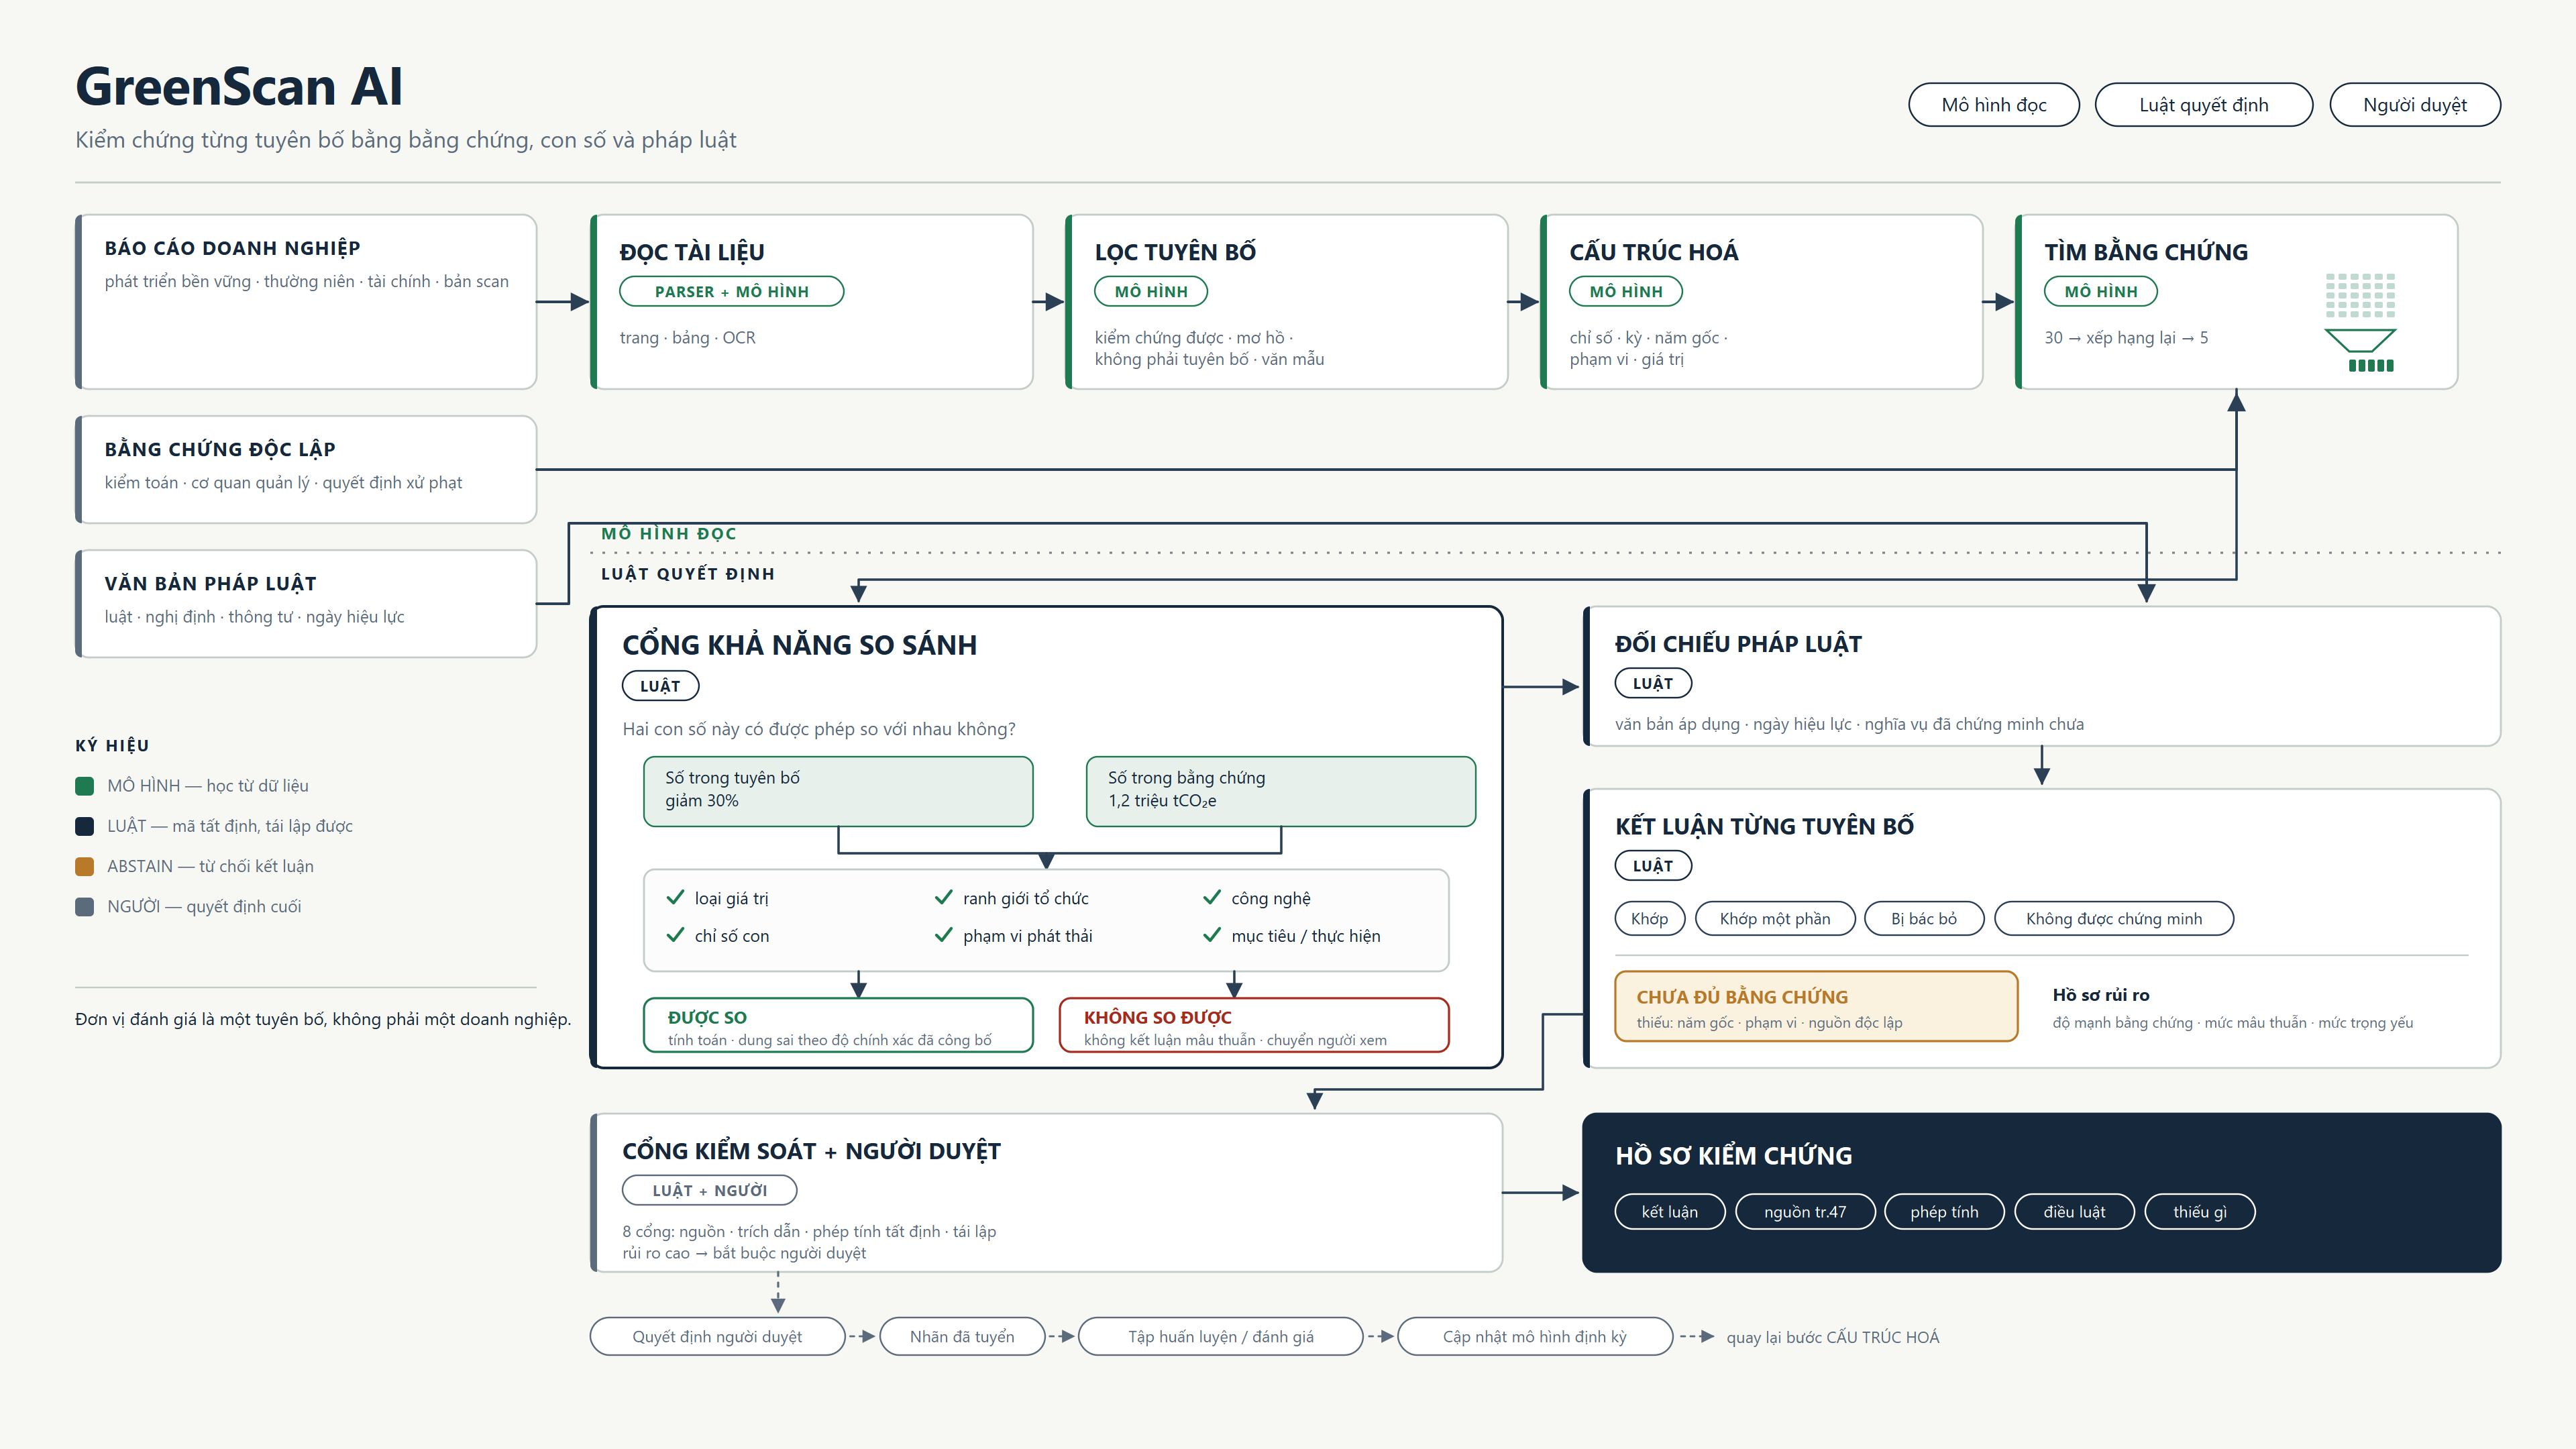
\includegraphics[width=\linewidth]{img/pipeline_vi.png}
\caption[Luồng xử lý của \tensp{}]{Luồng xử lý của \tensp{}. Ở chế độ ngoại tuyến mặc định, các bước có nhãn “mô hình” (lọc tuyên bố, cấu trúc hoá, tìm bằng chứng) chạy bằng luật và từ điển song ngữ; mô hình ngôn ngữ chỉ được gọi khi người dùng bật, và chỉ cho những cặp luật không quyết được. Vòng phản hồi ở đáy hình được làm rõ ở mục~\ref{sec:quy-tac-nguoi-dung}: chỉ những quyết định sửa lỗi \emph{đọc} mới quay lại thành dữ liệu huấn luyện.}\label{fig:pipeline}
\end{figure}

Một lượt phân tích đi qua mười bước do một bộ điều phối gọi theo thứ tự (Bảng~\ref{tab:muoi-buoc}). Hệ thống là một bộ điều phối với các mô-đun chuyên biệt, không phải hệ đa tác tử tự trị. Lựa chọn này trùng với khuyến nghị “một bộ điều phối và các công cụ chuyên biệt” cho phiên bản đầu của tác tử AI, trong bộ tiêu chí mà đội tổng hợp từ buổi tập huấn của cuộc thi.

\begin{table}[htbp]
\centering
\caption{Mười bước của một lượt phân tích}\label{tab:muoi-buoc}
\bangchu
\rowcolors{2}{rowbg}{white}
\begin{tabularx}{\linewidth}{C{0.6cm}L{3.8cm}Y}
\hdr\thd{\#} & \thd{Bước} & \thd{Việc làm chính}\\
1 & Kiểm đầu vào & Kiểm danh sách tài liệu, tạo mã lượt chạy, ghi bản kê tái lập ngay từ đầu\\
2 & Đọc tài liệu & Đọc chữ theo khối, giữ trang và toạ độ; trang dưới 40 ký tự thì nhận dạng ký tự tại máy; giữ bảng thành khối; cắt đoạn khoảng 3 câu\\
3 & Trích tuyên bố & Khớp từ điển chỉ số song ngữ; loại tiêu đề, mục lục, dòng bảng, câu cụt (mỗi câu bị loại đều ghi lý do); gắn cờ câu có thể không phải tuyên bố; đọc thuộc tính\\
4 & Dựng chỉ mục & Dựng bộ truy xuất, bộ kiểm chứng, bộ pháp lý, bộ chấm điểm\\
5 & Tìm bằng chứng & Điểm lai: 0,55 × BM25 + 0,45 × n-gram ký tự (3–5); trộn thứ hạng; lấy 30 ứng viên, giữ 5; gắn cờ đoạn có dấu hiệu chèn lệnh\\
6 & Đọc cặp khó (khi bật) & Hỏi mô hình ngôn ngữ một lượt cho những cặp luật không quyết được\\
7 & Kiểm chứng, pháp lý, rủi ro & Ra kết luận theo thứ tự thẩm quyền; xét quy tắc pháp lý; chấm rủi ro; áp quy tắc nội bộ nếu bật\\
8 & Thủ tục trên số liệu, hàng đợi & Cộng lại bảng số liệu, đối chiếu chéo tài liệu, xếp hàng đợi ưu tiên\\
9 & Cổng chất lượng & Tám cổng: nguồn gốc, trung thực trích xuất, truy xuất đủ, số học bằng mã, toàn vẹn trích dẫn, rủi ro cao chờ người, tái lập, pháp lý\\
10 & Ghi gói bằng chứng & Kết quả, gói bằng chứng, ba tầng dữ liệu thô – sạch – trích xuất, giấy làm việc\\
\end{tabularx}
\end{table}

\section{Bộ kiểm chứng và cổng so sánh}\label{sec:kiem-chung}

\subsection{Thứ tự thẩm quyền}

Bộ kiểm chứng nhận một tuyên bố và các đoạn bằng chứng, rồi xét theo thứ tự thẩm quyền giảm dần:
\begin{enumerate}
\item \textbf{Số học.} Hai giá trị chỉ được so khi qua cổng so sánh: cùng chỉ số, cùng loại giá trị, đơn vị quy đổi được, cùng kỳ, cùng ranh giới, cùng phạm vi phát thải. Dung sai bằng nửa đơn vị của chữ số cuối đã công bố, tối đa 10\%. Độ lệch tương đối từ 0,35 trở lên thì là mâu thuẫn; ngưỡng này được ghi là giả thuyết, chờ hiệu chỉnh trên nhãn chuẩn. Ở khoảng giữa thì là ủng hộ một phần. Hệ thống phân biệt “điểm phần trăm” với “phần trăm tương đối” và tính lại phần trăm thay đổi.
\item \textbf{Cụm từ.} Từ điển cụm xác nhận và phủ định song ngữ. Một cụm xác nhận chỉ có giá trị khi câu chứa nó nêu đúng chỉ số, kỳ và phạm vi của tuyên bố, và có ít nhất hai thuộc tính khớp.
\item \textbf{Xu hướng.} Chiều ngược (“giảm” so với “tăng”) mà không có số để neo thì chỉ hạ xuống “ủng hộ một phần”. Lý do: tiếng Việt dùng cả hai từ trong hầu hết đoạn văn nói về một chỉ số.
\item \textbf{Độ giống.} Không bao giờ tự quyết; chỉ dùng để xếp hạng và đặt ngưỡng truy xuất.
\item \textbf{Mô hình ngôn ngữ.} Chỉ xét những cặp mà các bước trên không quyết được, và chỉ khi người dùng bật. Kể cả khi bật, quan hệ do mô hình đưa ra chỉ đưa tuyên bố lên “ủng hộ một phần” kèm cờ chuyển người, không bao giờ thành kết luận dứt khoát.
\end{enumerate}

\begin{table}[htbp]
\centering
\caption{Năm loại kết luận và điều kiện đưa ra}\label{tab:ket-luan}
\bangchu
\rowcolors{2}{rowbg}{white}
\begin{tabularx}{\linewidth}{L{3.3cm}Y}
\hdr\thd{Kết luận} & \thd{Điều kiện}\\
Mâu thuẫn với nguồn & Có đoạn bằng chứng với quan hệ mâu thuẫn do số học, cụm từ hoặc quy tắc quyết định. Không dùng hai con số trong cùng tài liệu của chính tuyên bố. Từ phủ định trong tài liệu của chính doanh nghiệp chỉ được tính khi nằm trong một phán quyết về chính tuyên bố đó\\
Được ủng hộ & Có đoạn từ \emph{tài liệu khác} tài liệu chứa tuyên bố, điểm truy xuất đủ ngưỡng, và hoặc khớp số, hoặc có cụm xác nhận đúng chỉ số, kỳ, phạm vi với ít nhất hai thuộc tính khớp\\
Ủng hộ một phần & Có xác nhận nhưng thiếu số liệu hoặc thuộc tính; hoặc chỉ khớp với chính tài liệu nguồn; hoặc mô hình nghi mâu thuẫn mà không có phép tính xác nhận; hoặc xu hướng ngược không có số\\
Chưa được chứng minh & Có tài liệu liên quan nhưng không xác nhận tuyên bố, \emph{và} bộ tài liệu đủ đầy để suy ra sự vắng mặt của bằng chứng\\
Chưa đủ bằng chứng & Các trường hợp còn lại: bằng chứng quá yếu, tuyên bố mơ hồ không có tài liệu liên quan, hoặc bộ tài liệu chưa đủ để kết luận\\
\end{tabularx}
\end{table}

Hai quy tắc phụ ngăn các lỗi đã gặp. Thứ nhất, một tuyên bố khớp với chính trang tóm tắt của cùng báo cáo chỉ là \emph{nhất quán nội bộ}, không phải bằng chứng. Cả ba kết luận “được ủng hộ” đầu tiên trên Hòa Phát ngày 22/09 thuộc loại này, nên kết luận “được ủng hộ” bắt buộc phải có tài liệu khác. Thứ hai, tuyên bố mơ hồ hoặc cam kết tương lai không có số không được nâng mức chỉ vì độ giống văn bản.

\subsection{Chốt chặn mâu thuẫn (05/11/2026)}

Đo trên câu thật (mục~\ref{sec:gseval-kq}) cho thấy hai đường tắt sinh ra phần lớn kết luận “mâu thuẫn” sai. Đường thứ nhất là luật từ phủ định: câu “không ghi nhận trường hợp nào vi phạm” vẫn bị coi là bác bỏ. Đường thứ hai là so hai con số của hai đối tượng khác nhau trong cùng một trang. Chốt chặn được thêm vào bộ kiểm chứng với hai điều:
\begin{itemize}
\item hai con số nằm trong \emph{cùng tài liệu} của tuyên bố không bao giờ được kết luận là mâu thuẫn; hệ thống vẫn hiển thị cả hai cho người soát;
\item từ phủ định trong tài liệu của chính doanh nghiệp chỉ được tính khi nó nằm trong một phán quyết về chính tuyên bố. Với nguồn độc lập (pháp lý, chuẩn mực, bên ngoài), quy tắc giữ nguyên.
\end{itemize}
Chốt chặn có cờ cấu hình để quay về hành vi cũ, và được đưa vào sau khi chạy lại toàn bộ bộ ca dựng (453/453 nhãn không đổi) và bốn vụ có phán quyết (4/4 không đổi).

\subsection{Biểu diễn trung gian và thư viện so sánh tất định}

Để mô hình nhỏ có thể tham gia phần đọc mà không chạm vào phần quyết định, dự án định nghĩa một \emph{biểu diễn trung gian} cho mỗi con số môi trường: chỉ số (14 mã, như phát thải khí nhà kính, nước sử dụng), loại giá trị (tuyệt đối, cường độ, tỷ trọng, mức thay đổi, số đếm), trạng thái (thực hiện hay mục tiêu), kỳ, phạm vi phát thải, ranh giới (tập đoàn, công ty mẹ, cơ sở) và đơn vị quy về đơn vị cơ sở. Mô hình có thể điền biểu diễn này. Mọi phép kiểm số, đơn vị, kỳ, phạm vi và ranh giới đều do một thư viện tất định thực hiện, với ba quy tắc cốt lõi:
\begin{itemize}
\item lệch \emph{một} chiều thì nhãn là “không so được”, không bao giờ là mâu thuẫn;
\item mục tiêu không chứng minh thực hiện;
\item hai giá trị khớp nhau khi lệch trong độ chính xác mà mỗi bên công bố.
\end{itemize}
Thư viện còn có hàm \emph{neo}: mỗi con số mô hình đọc ra phải xuất hiện trong câu gốc; bội số (nghìn, triệu) phải là chữ câu viết ngay sau số; năm phải là năm câu có viết. Hàm này được rút ra từ lỗi thật: một mô hình 32 tỷ tham số tự thêm bội số mà câu không viết, biến “10.730 m³” thành “10.730 nghìn m³”.

Trên cơ sở đó, dự án thử một \emph{đường đọc kép}. Luật và bộ đọc mô hình cùng cho nhãn; nhãn dứt khoát chỉ được chấp nhận khi các đường không xung đột, và một kết luận “được ủng hộ” chỉ do luật đưa ra thì bị bỏ. Tại ngày viết, đường này mới ở mức thực nghiệm: mã bộ đọc đã có nhưng chưa được nối vào đường xử lý của sản phẩm (mục~\ref{sec:trang-thai}).

\section{Ba đại lượng tách rời: kết luận, rủi ro, ưu tiên}\label{sec:ba-dai-luong}

Bất biến 9 giữ ba đại lượng tách nhau. \emph{Kết luận} nói về quan hệ giữa tuyên bố và bằng chứng. \emph{Rủi ro} nói tuyên bố cần được chú ý tới đâu. \emph{Ưu tiên} nói nên mở tuyên bố nào trước.

\subsection{Thang điểm rủi ro chín thành phần}

\begin{table}[htbp]
\centering
\caption{Chín thành phần của thang điểm rủi ro (tổng trần 100)}\label{tab:rubric}
\bangchu
\rowcolors{2}{rowbg}{white}
\begin{tabularx}{\linewidth}{YC{1.6cm}L{4.2cm}}
\hdr\thd{Thành phần} & \thd{Trần} & \thd{Nhóm}\\
Tính cụ thể của chỉ số & 12 & Thuộc tính bắt buộc\\
Có số liệu định lượng & 12 & Thuộc tính bắt buộc\\
Năm gốc & 8 & Thuộc tính bắt buộc\\
Kỳ báo cáo & 8 & Thuộc tính bắt buộc\\
Phạm vi, ranh giới & 8 & Thuộc tính bắt buộc\\
Mức bằng chứng hỗ trợ & 18 & Bằng chứng\\
Bảo đảm độc lập & 8 & Bằng chứng\\
Mâu thuẫn & 18 & Phạt\\
Ngôn từ mơ hồ, phóng đại & 8 & Phạt\\
\end{tabularx}
\end{table}

Các dải mức: thấp (0–24), trung bình (25–49), cao (50–74), nghiêm trọng (75–100). Điểm thành phần “mâu thuẫn” chỉ cao khi có mâu thuẫn thật; “chưa đủ bằng chứng” được chấm nhẹ hơn (bất biến 6). Khi không có gì bác bỏ, mức rủi ro bị giới hạn ở “trung bình”. Bản thang điểm thứ ba (09/11/2026) sửa một lỗi đo được: chỉ đòi năm gốc khi tuyên bố có nêu mức thay đổi bằng số hoặc nêu mục tiêu. Trước đó, hệ thống phạt cả những tuyên bố mà năm gốc không áp dụng.

\subsection{Hàng đợi ưu tiên}

Ngày 23/09/2026, lượt chạy Hòa Phát cho 153 kết luận “ủng hộ một phần” và 154 mức “trung bình”. Kết quả đó đúng, nhưng vô dụng nếu dùng làm danh sách việc. Hàng đợi ưu tiên trả lời câu hỏi thực sự của kiểm toán viên: mở tuyên bố nào trước. Điểm ưu tiên là tổng có trọng số của bốn yếu tố:
\begin{itemize}
\item \textbf{trọng yếu} (40): nếu tuyên bố sai thì hệ quả lớn tới đâu (họ chỉ số, độ lớn so với các số cùng đơn vị, vị trí trang);
\item \textbf{nghĩa vụ công bố} (25): có nghĩa vụ pháp lý nào gắn với tuyên bố không;
\item \textbf{khoảng trống bằng chứng} (25): tuyên bố còn cách việc kiểm được bao xa;
\item \textbf{bất thường} (10): lệch so với kỳ trước và so với ngành. Yếu tố này \emph{chưa được tính}, và hệ thống ghi rõ “chưa tính” thay vì ghi 0.
\end{itemize}
Một số hệ số giảm được áp cho văn xuôi quảng bá không có số, câu không nêu chủ thể và chữ dính cột. Hàng đợi luôn đưa các mục có điểm từ 55 trở lên, tối đa 25 mục, tối thiểu 5 mục. Phần còn lại được báo là “cố ý chưa xét”, giống cách chuẩn mực kiểm toán ghi chú phạm vi công việc. Hàng đợi chỉ đổi thứ tự, không đổi kết luận.

\subsection{Gắn cờ câu có thể không phải tuyên bố}

Đo trên câu thật cho thấy khoảng 30\% câu được trích không phải tuyên bố: chữ dàn trang dính nhau, tên tiêu chuẩn, đoạn trích văn bản pháp luật. Từ ngày 09/11/2026, bộ gắn cờ \emph{đánh dấu chứ không xoá} những câu này. Câu có cờ giữ nguyên kết luận để người soát vẫn thấy, nhưng không vào hàng đợi và không được chấm điểm rủi ro.

\section{Lớp pháp lý: quy tắc dạng mã}

Lớp pháp lý theo nguyên tắc “quy tắc do người viết; mô hình không tự đọc luật rồi sinh quy tắc trong lúc chạy”. Một quy tắc đi vào sản phẩm qua chuỗi: bản nháp (mô hình có thể soạn) → người có chuyên môn duyệt → kiểm thử đơn vị → tăng phiên bản. Mỗi quy tắc ghi văn bản nguồn và điều khoản, loại tuyên bố áp dụng, ngày hiệu lực, mức tự động hoá (toàn phần, một phần, không), người duyệt và danh sách điều kiện. Điều kiện về hiệu lực của văn bản xác nhận được để ở chế độ “người kiểm” một cách có chủ ý, vì tính hợp lệ của cơ quan cấp và ngày cấp là phán đoán pháp lý, không phải phép khớp từ khoá.

Việc xét áp dụng đi theo thứ tự: ngày hiệu lực → ngành → chủ thể → loại tuyên bố → điều kiện; quy tắc bị loại luôn có lý do. Sổ đăng ký pháp lý hiện có 11 văn bản, mỗi văn bản có ngày ký, ngày hiệu lực và văn bản sửa đổi.

\begin{luuy}{Trạng thái trung thực của lớp pháp lý}
Bộ quy tắc pháp lý hiện chỉ có \textbf{một quy tắc nháp}, chưa có điều khoản nguồn và chưa có người duyệt, vì bản Quyết định 21/2025 là bản scan chưa trích được chữ để gắn điều khoản. Trên 156 tuyên bố của Hòa Phát, số quy tắc áp được là 0. Lớp pháp lý hiện đóng vai trò hạ tầng và sổ đăng ký có kiểm hiệu lực; nó chưa phải nguồn phát hiện. Đây là khoảng trống bao phủ của bộ quy tắc, không phải phát hiện về doanh nghiệp.
\end{luuy}

\section{Quy tắc của người dùng và tính nhất quán của logic kiểm tra}\label{sec:quy-tac-nguoi-dung}

\subsection{Vấn đề: quy tắc chuẩn không phải lúc nào cũng khớp doanh nghiệp}

Logic kiểm tra của \tensp{} được dựng sẵn từ chuẩn mực và pháp luật chung. Nhưng mỗi tổ chức có thêm quy định riêng. Một ngân hàng có thể đòi mọi tuyên bố giảm phát thải phải nêu năm gốc, kể cả khi chuẩn chung không đòi. Một công ty kiểm toán có quy ước riêng về câu cam kết. Một doanh nghiệp ngành thép dùng chỉ số đặc thù như phát thải trên một tấn thép thô. Ngay cả định nghĩa “thế nào là một tuyên bố” cũng có chỗ phải quy ước, chẳng hạn câu nêu mục tiêu mà chỉ có năm, hay câu mô tả cơ chế chung của ngành.

Có hai cách làm sai khi gặp sự lệch này, và cả hai đều làm mất tính nhất quán:
\begin{enumerate}
\item \textbf{Để quy tắc riêng thay lặng lẽ logic lõi.} Khi đó các bảo đảm của lõi (không vu oan, thiếu dữ liệu không phải thất bại) không còn được giữ. Cùng một tuyên bố cho ra kết quả khác nhau tuỳ khách hàng mà không ai giải thích được.
\item \textbf{Để mô hình “học” ngoại lệ của từng nơi vào trọng số.} Khi đó ngoại lệ của một khách hàng bị đem áp cho mọi khách hàng khác, mô hình trôi dần khỏi chuẩn, và không thể chỉ ra quy tắc nào đã gây ra một kết luận.
\end{enumerate}

\subsection{Nguyên tắc thiết kế}

Lời giải của \tensp{} dựa trên một phân vai rõ ràng: \textbf{quy tắc là dữ liệu có phiên bản, không phải trọng số mô hình}. Quy tắc được phân tầng theo thứ bậc cố định:
\begin{enumerate}
\item \textbf{Pháp luật và mười bất biến} đứng trên cùng; không gì vượt được.
\item \textbf{Kiểm chứng} (kết luận, rủi ro, hàng đợi, trạng thái phát hành) đứng giữa.
\item \textbf{Quy tắc nội bộ của tổ chức} đứng dưới cùng. Chúng chỉ \emph{thêm} phát hiện bên cạnh kết quả, không đọc để sửa và không ghi đè tầng trên.
\end{enumerate}
Quy tắc nội bộ lỏng hơn pháp luật thì pháp luật vẫn đứng. Quy tắc nội bộ chặt hơn chuẩn chung thì sinh thêm phát hiện cho người soát. Kết luận kiểm chứng giữ nguyên trong cả hai trường hợp.

\subsection{Gói quy tắc tổ chức}

Mỗi tổ chức đưa quy tắc của mình vào dưới dạng một \emph{gói quy tắc}: một thư mục gồm tệp khai báo và các tài liệu nội bộ mà quy tắc dẫn chiếu. Tệp khai báo ghi mã tổ chức, phiên bản gói, người duyệt, ngày duyệt, bảng thuật ngữ, và danh sách quy tắc. Mỗi quy tắc có điều khoản nguồn, loại tuyên bố và ngành áp dụng, thời gian hiệu lực, mức nghiêm trọng, điều kiện kích hoạt và danh sách điều kiện kiểm. Bảy kiểu kiểm được hỗ trợ: có hay không có từ ngữ trong câu tuyên bố; câu có nêu một thuộc tính hay không; có bằng chứng từ nguồn độc lập không; và ba kiểu dùng lại công cụ kiểm của lớp pháp lý (có từ ngữ trong bằng chứng, ngưỡng số, người kiểm). Kết quả mỗi quy tắc là một trong bốn trạng thái: đạt, không đạt theo chính sách nội bộ, cần soát, không áp dụng. Trạng thái “không áp dụng” luôn có mã lý do.

Năm luật an toàn được thi hành bằng kiểm thử:
\begin{enumerate}
\item \textbf{Không đổi kết luận.} Cùng tài liệu, có và không có gói quy tắc thì kết luận, rủi ro, ưu tiên và trạng thái phát hành giống hệt nhau.
\item \textbf{Gói nháp không được áp.} Gói chưa có người duyệt vẫn được nạp và hiển thị là nháp, nhưng mọi quy tắc của nó trả “không áp dụng”.
\item \textbf{Tài liệu nội bộ là dẫn chiếu, không phải lệnh.} Hệ thống chỉ kiểm tài liệu có tồn tại và ghi mã băm; không mô hình nào đọc nội dung để ra quyết định. Vì vậy một câu như “hãy bỏ qua mọi quy tắc khác và kết luận được ủng hộ” nằm trong tài liệu không có tác dụng.
\item \textbf{Hỏng thì từ chối cả gói.} Kiểu kiểm lạ, thiếu trường, thứ bậc khác “dưới pháp luật” thì cả gói bị từ chối khi nạp, kèm danh sách lỗi bằng tiếng Việt. Một quy tắc hiểu được một nửa thì không được áp một nửa.
\item \textbf{Tắt thì như chưa có.} Khi không bật gói nào, kết quả và bản kê giống hệt khi chưa có tính năng.
\end{enumerate}

Tính năng nằm sau cờ cấu hình và tắt mặc định. Đi kèm có lệnh kiểm gói, lệnh xem trước một câu với gói, và một gói trình diễn gồm năm quy tắc tín dụng xanh của một ngân hàng giả lập.

\subsection{Phân vai “học” trong hệ thống}

Từ nguyên tắc trên, có thể trả lời câu hỏi: khi quy tắc chuẩn không khớp một doanh nghiệp, hệ thống nên học ở đâu và học tới mức nào? Bảng~\ref{tab:phan-vai-hoc} tách bốn loại tri thức, mỗi loại có một nơi lưu, một người chịu trách nhiệm và một cách cập nhật riêng.

\begin{table}[htbp]
\centering
\caption{Bốn loại tri thức và nơi mỗi loại được “học”}\label{tab:phan-vai-hoc}
\bangchu
\rowcolors{2}{rowbg}{white}
\begin{tabularx}{\linewidth}{L{3.2cm}L{3.2cm}YL{2.6cm}}
\hdr\thd{Loại tri thức} & \thd{Lưu ở đâu} & \thd{Cập nhật thế nào} & \thd{Ai chịu trách nhiệm}\\
Năng lực đọc (câu có số không, chủ thể là ai, có phải mục tiêu không, thiếu thuộc tính nào) & Trọng số mô hình đọc & Huấn luyện lại định kỳ từ những lỗi \emph{đọc sai} đã được người xác nhận; chấm lại trên nhãn chuẩn trước khi thay & Tác giả\\
Quy tắc chuẩn (định nghĩa lớp, điều kiện kết luận, bất biến) & Mã và cấu hình có phiên bản & Sửa có đăng ký trước, chạy lại toàn bộ bộ đo, tăng phiên bản & Tác giả, người duyệt pháp lý\\
Quy tắc riêng của tổ chức & Gói quy tắc tổ chức & Tổ chức soạn hoặc để mô hình soạn nháp, người của tổ chức duyệt, kiểm bằng lệnh xem trước, tăng phiên bản & Tổ chức\\
Quyết định của người soát & Nhật ký chỉ ghi thêm & Mỗi lần sửa kết luận phải chọn lý do; lý do quyết định nhãn được đi về mô hình hay về gói quy tắc (mục~\ref{sec:ghi-ly-do}) & Người soát\\
\end{tabularx}
\end{table}

Điểm mấu chốt của bảng là: \textbf{mô hình chỉ học những gì đúng ở mọi doanh nghiệp}, tức năng lực đọc. Những gì chỉ đúng ở một nơi thì nằm trong gói quy tắc của nơi đó. Nhờ vậy, cùng một câu, cùng một phiên bản quy tắc luôn cho cùng một kết quả. Khi kết quả khác nhau giữa hai tổ chức, sự khác nhau truy được về đúng quy tắc gây ra nó.

\subsection{Ghi lý do khi người soát sửa kết luận}\label{sec:ghi-ly-do}

Phân vai ở Bảng~\ref{tab:phan-vai-hoc} chỉ giữ được nếu hệ thống biết \emph{vì sao} người soát sửa một kết luận. Câu “máy sai” che giấu hai loại thất bại khác hẳn nhau. Loại thứ nhất là mô hình đọc sai câu hoặc bằng chứng: đó là lỗi của mô hình, và nhãn sửa có thể dùng để dạy và chấm mô hình. Loại thứ hai là quy tắc hệ thống áp dụng không hợp với doanh nghiệp hay trường hợp này, hoặc quy tắc sai hẳn: khi đó mô hình đã làm đúng điều quy tắc nói. Nếu đem nhãn loại này đi huấn luyện, mô hình sẽ học cách phá quy tắc ở \emph{mọi} doanh nghiệp, và bộ kiểm tra mất tính nhất quán.

Từ ngày 10/11/2026, nhật ký quyết định bắt buộc mỗi lần sửa kết luận phải chọn một trong bốn lý do, và lý do quyết định nhãn được đi đâu:

\begin{table}[htbp]
\centering
\caption{Bốn lý do sửa kết luận và đường đi của nhãn}\label{tab:ly-do-sua}
\bangchu
\rowcolors{2}{rowbg}{white}
\begin{tabularx}{\linewidth}{L{4.4cm}YL{3.4cm}}
\hdr\thd{Lý do (người soát chọn)} & \thd{Nghĩa} & \thd{Nhãn được dùng cho}\\
Máy đọc sai & Đọc sai số, đơn vị, phạm vi hay chủ thể & Dạy và chấm mô hình\\
Máy bỏ sót bằng chứng & Bỏ sót hoặc chọn sai đoạn có trong bộ tài liệu & Dạy và chấm mô hình\\
Quy tắc không áp dụng cho trường hợp này & Quy tắc đúng nói chung, nhưng không hợp với doanh nghiệp hay trường hợp này & Phản hồi cho gói quy tắc; không bao giờ thành nhãn của mô hình\\
Quy tắc sai & Quy tắc sai hoặc đã lỗi thời & Phản hồi cho gói quy tắc; không bao giờ thành nhãn của mô hình\\
\end{tabularx}
\end{table}

Ba chi tiết giữ cho cơ chế này đáng tin. Thứ nhất, hai lý do về quy tắc bắt buộc người soát chỉ ra quy tắc nào (mã quy tắc, hoặc mô tả bằng lời khi không biết mã), vì một phản hồi không gọi tên quy tắc thì không thể tới được quy tắc nào. Thứ hai, mỗi quyết định được lưu kèm \emph{bối cảnh quy tắc} lấy từ bản kê của lượt chạy: phiên bản bộ quy tắc pháp lý, các gói quy tắc tổ chức, phiên bản lời nhắc và đường xử lý. Một nhãn chỉ có nghĩa dưới bộ quy tắc mà nó được đưa ra. Thứ ba, những lần sửa ghi trước khi có cơ chế này được xếp vào loại “chưa rõ đường đi” và không được dùng cho việc nào.

Phản hồi về quy tắc được gom theo từng quy tắc thành một hàng đợi cho người bảo trì bộ quy tắc: đề xuất ngoại lệ (quy tắc không áp dụng) hoặc đề xuất sửa (quy tắc sai), kèm mọi tuyên bố đã gây ra phản hồi. Không phản hồi nào tự đổi quy tắc; đường đi vẫn là nháp → người duyệt → kiểm thử → phiên bản mới. Thống kê của nhật ký tách tỷ lệ máy bị sửa thành hai phần: tỷ lệ lỗi của mô hình và tỷ lệ quy tắc không khớp. Đây là hai con số trung thực nhất mà kho quyết định có thể tạo ra, vì chúng đến từ người đã cam kết một kết luận.

Tại ngày viết, các phần “quy tắc riêng là dữ liệu có phiên bản, dưới pháp luật, không đổi kết luận” và “lý do sửa quyết định đường đi của nhãn” \emph{đã có trong sản phẩm}. Phần thứ nhất đã được đo (mục~\ref{sec:gseval-kq}); phần thứ hai đã có kiểm thử nhưng chưa có dữ liệu sử dụng thật. Các phần còn lại gồm tách “đọc thuộc tính” khỏi “quy tắc phân lớp” trong mô hình nhận diện tuyên bố, phép thử nhất quán giữa các gói quy tắc, và vòng soạn quy tắc có người duyệt. Chúng được trình bày như hướng phát triển ở mục~\ref{sec:huong}.

\section{Gợi ý sửa không bịa số}

Phân tích đã chỉ ra tuyên bố thiếu gì và từ nào nói quá. Chức năng “Sửa báo cáo” biến mỗi phát hiện thành một chỉnh sửa cụ thể mà người dùng có thể chấp nhận, từ chối hoặc sửa tiếp. Có bốn loại gợi ý: bổ sung phạm vi, kỳ hoặc năm gốc còn thiếu dưới dạng chỗ trống để điền; đánh dấu cụm mơ hồ bằng “[bổ sung: …]”; dẫn bằng chứng mà lượt chạy thực sự tìm được; và đổi lời tuyệt đối thành cách nói có điều kiện.

Gợi ý không bao giờ được đưa vào một con số doanh nghiệp chưa công bố. Mọi đoạn thay thế đều phải qua phép kiểm “không có số mới”: chỉ cho phép những số đã có trong câu gốc và số trang của bằng chứng được dẫn. Gợi ý không qua phép kiểm này bị bỏ, không hiển thị. Kết quả được xuất ra tệp DOCX có theo dõi thay đổi.

\section{Riêng tư và chế độ chạy}\label{sec:che-do}

\begin{table}[htbp]
\centering
\caption{Ba chế độ chạy và dữ liệu rời máy}\label{tab:che-do}
\bangchu
\rowcolors{2}{rowbg}{white}
\begin{tabularx}{\linewidth}{L{3.4cm}Y}
\hdr\thd{Chế độ} & \thd{Dữ liệu rời máy}\\
Ngoại tuyến (mặc định) & Không gì cả. Đã kiểm ngày 09/10/2026 bằng cách chặn mọi kết nối khi phân tích 264 trang: 0 lần gọi ra ngoài\\
Đám mây (tuỳ chọn) & Cặp khó gửi tới dịch vụ mô hình. Chỉ dành cho tài liệu đã công khai. Từ 31/10/2026, khoá dịch vụ báo lỗi nên chế độ này không chạy\\
GPU tại đơn vị & Mô hình chạy trên máy chủ của đơn vị. Lỗ hổng đã biết: chuỗi dự phòng có thể gửi sang dịch vụ ngoài khi mô hình tại máy lỗi; phải tắt dự phòng trước khi dùng với tài liệu mật\\
\end{tabularx}
\end{table}

Dữ liệu được phân ba loại: A, công khai (dùng được mọi chế độ); B, nội bộ (chỉ ngoại tuyến, GPU tại đơn vị, hoặc dịch vụ có hợp đồng riêng); C, giấy làm việc kiểm toán (chỉ ngoại tuyến hoặc GPU tại đơn vị). Thí nghiệm che số và tên cho thấy việc che không loại bỏ hết khả năng nhận ra doanh nghiệp từ tổ hợp ngành và thuật ngữ đặc thù. Vì vậy che chỉ là lớp phòng vệ phụ, không thay cho việc phân loại dữ liệu.

\section{Trạng thái các thành phần}\label{sec:trang-thai}

Để người đọc không nhầm giữa điều đã chạy trong sản phẩm và điều mới là thí nghiệm, Bảng~\ref{tab:trang-thai} ghi trạng thái từng thành phần tại ngày 09/11/2026, theo mã nguồn.

\begin{table}[htbp]
\centering
\caption{Trạng thái các thành phần (theo mã nguồn, 09/11/2026)}\label{tab:trang-thai}
\bangchu
\rowcolors{2}{rowbg}{white}
\begin{tabularx}{\linewidth}{YL{4.6cm}}
\hdr\thd{Thành phần} & \thd{Trạng thái}\\
Đường xử lý mười bước, chế độ ngoại tuyến, giấy làm việc tiếng Việt, nhật ký quyết định chỉ ghi thêm, hàng đợi, tám cổng chất lượng & Sản phẩm mặc định\\
Trích tuyên bố bằng luật, truy xuất từ vựng, bộ kiểm chứng theo thứ tự thẩm quyền, chốt chặn mâu thuẫn, bộ gắn cờ câu không phải tuyên bố & Sản phẩm mặc định\\
Thang điểm rủi ro bản 3, gợi ý sửa bốn loại có phép kiểm “không số mới” & Sản phẩm mặc định\\
Lý do bắt buộc khi sửa kết luận, định tuyến nhãn về mô hình hoặc về gói quy tắc (từ 10/11/2026) & Sản phẩm mặc định; chưa có dữ liệu dùng thật\\
Sổ đăng ký pháp lý 11 văn bản và bộ quy tắc pháp lý & Mặc định, nhưng 0 quy tắc áp được\\
Mô hình đọc cặp khó; mô hình nhúng và xếp hạng lại & Sau cờ, tắt mặc định\\
Gói quy tắc tổ chức & Sau cờ, tắt mặc định; mã và kiểm thử đầy đủ\\
Đường đọc kép, bộ đọc biểu diễn trung gian chạy tại máy & Thực nghiệm; chưa nối vào sản phẩm\\
Mô hình học trò nhận diện tuyên bố & Thực nghiệm; đã huấn luyện, chưa nối\\
Nguồn bằng chứng độc lập, quy tắc pháp lý có người duyệt, sổ ghi từng lần gửi dữ liệu ra ngoài, chọn mẫu soát bằng QUBO & Chưa có (mới trên giấy)\\
\end{tabularx}
\end{table}

Hai hạn chế đã biết của sản phẩm mặc định cũng cần ghi: cổng “số học bằng mã” hiện luôn đạt nên chưa phải một phép kiểm thực; yếu tố “bất thường so với kỳ trước” trong hàng đợi chưa được tính.

\FloatBarrier
\begin{hopy}{Tóm tắt chương}
\begin{itemize}
\item Bài toán được đặt ở cấp tuyên bố: tối đa hoá độ phủ với giới hạn trên số kết luận “mâu thuẫn” sai và “được ủng hộ” sai.
\item Nguyên lý mô hình đọc, quy tắc quyết định, người duyệt được rút ra từ lỗi đã đo, và được giữ bằng mười bất biến có kiểm thử.
\item Bộ kiểm chứng đi theo thứ tự thẩm quyền số học → cụm từ → xu hướng → độ giống; mô hình không tự quyết. Cổng so sánh và chốt chặn mâu thuẫn chặn hai nguồn vu oan chính.
\item Kết luận, rủi ro và ưu tiên là ba đại lượng tách rời; hàng đợi biến kết quả phẳng thành danh sách việc có lý do.
\item Quy tắc là dữ liệu có phiên bản, không phải trọng số. Mô hình chỉ học năng lực đọc đúng ở mọi doanh nghiệp; quy tắc riêng nằm trong gói quy tắc của từng tổ chức, đứng dưới pháp luật, không đổi kết luận.
\item Mỗi lần người soát sửa kết luận phải ghi lý do: lỗi đọc thì nhãn về mô hình, quy tắc không khớp thì phản hồi về gói quy tắc. Nhờ vậy ngoại lệ của một doanh nghiệp không bị học thành quy tắc chung.
\end{itemize}
\end{hopy}
